\newif\ifpdf
\ifx\pdfoutput\undefined
\pdffalse % we are not running PDFLaTeX
\else
\pdfoutput=1 % we are running PDFLaTeX
\pdftrue
\fi

\documentclass[a4paper]{article}
\usepackage[swedish, english]{babel}
\usepackage[T1]{fontenc}

\ifpdf
\usepackage[pdftex]{graphicx}
\renewcommand{\encodingdefault}{T1}
\renewcommand{\rmdefault}{pad}
\pdfcompresslevel=9
\else
\usepackage{graphicx}
\fi

%\usepackage{psfrag}
\usepackage{lscape}
\usepackage{rotating}
\usepackage{url}                      % (handy if you reference a URL.)
\makeatletter
\def\url@leostyle{
  \@ifundefined{selectfont}{\def\UrlFont{\sf}}{\def\UrlFont{\small\ttfamily}}}
\makeatother
\urlstyle{leo}
\usepackage{fancyhdr}
\pagestyle{fancy}
\lhead{\small{\textit{Frisk / Bullock}}}
\chead{}
\rhead{\small{\textit{The Integra Environment}}}

\usepackage{verbatim}

\title{Suggestions for the Integra Environment - Update.}
\author{\small{Jamie Bulloock, Henrik Frisk}}
\date{\today}

\begin{document}
\selectlanguage{english}
\maketitle

\thispagestyle{empty}
\section*{Summary of IRC meeting April 7, 2006}
\subsection*{participants: Jamie Bullock and Henrik Frisk}

The main thread in the meeting was what is referred to in the proposal
by Malm� Academy
({\url{http://www.integralive.org/Members/henrikf/suggestions-for-the-
integra-\environment/folder_contents}}) as the 'score' file. In other
words the structure of the data that is passed to modules by value. It
seems as if there has been no objections against using an XML file
format for this purpose. The discussion was only concerned with
terminology and structure and not at all about implementation - how
events/sequences/structures are to be read/written/sch\-eduled/dispatched.

The idea of splitting this data over different files, perhaps even
one per module, was discussed (this is the approach used by Jamoma). This
would mean that each module had its own list of possible 'states' and 'behaviours'
associated with it. These could be static (as in a preset) or they could
be gestures or patterns that change over time. They could also affect or
alter the behaviour of other modules. These XML files act as 'containers'
of information about module behaviours. Metaphorically speaking these
are the 'players' of the system. These 'players' can be nested into
'groups' in which they interact with each other following a 'conductor'
which is a container of meta information about the music (basically the
score). 

The 'player', the 'group' and the 'conductor' all have the same
function, but at different layers of the system. It is anticipated that
they would all support the same basic data types. Examples might
include, scalars, lists, arrays and hashes. However, a container should
only use types supported by the module with which it is
associated. Players, groups and conductors could be thought of as
instances of the container class. See fig. 1 for an approximation of how
the concept might work.

The advantage of using an approach in which this data is split up in
many files is that a set of 'behaviours' can be stored and updated along
with a module; 'the player' (the XML container) has an instrument (the
synthesis module) and knowledge about how to play it (the data in the
container). Technically, parsing the data will also be easier and
faster compared to a solution in which all of this data is stored in
one big file.

The possibility of integrating SMIL was also discussed. Though there are
interesting possibilities with this approach, it was decided that the
main priority now is to consolidate a basic XML specification for the
containers so we can begin development. SMIL could then be
incorporated at a later stage and form a subset to the Integra
XML container specification. 

Following is an example of a module specific XML file. In the example it
is assumed that it's possible to interpolate between all the parameters
in a module's preset using the same mode (linearly,
logarithmically...). One issue that has to be further discussed also in
relation to the OSC namespace is voice instantiation. Should it be
assumed that all synthesis modules is capable of producing  multiple
voices and in that case, what is the procedure for communicating control
data to just one of these voices?

The XML file structure has its head and body tags. In the body tag there
are three major sections:
\begin{itemize}
 \item The {\small \texttt{preset}} tag.
 \item The {\small \texttt{current}} tag.
 \item The {\small \texttt{synchro}} tag.
\end{itemize}
The contents of the {\small \texttt{preset}} tag communicates data \emph{to} the module,
the {\small \texttt{current}} tag receives information \emph{from} the module about its
current state and the {\small \texttt{synchro}} tag synchronizes the sending of data from
the player container to the module. The contents of the {\small \texttt{current}} tag
can also be referenced from the {\small \texttt{synchro}} tag.

{\small \verbatiminput{player.xml} }
%\begin{center}
%\begin{landscape}
\begin{sidewaysfigure} %[ptb]
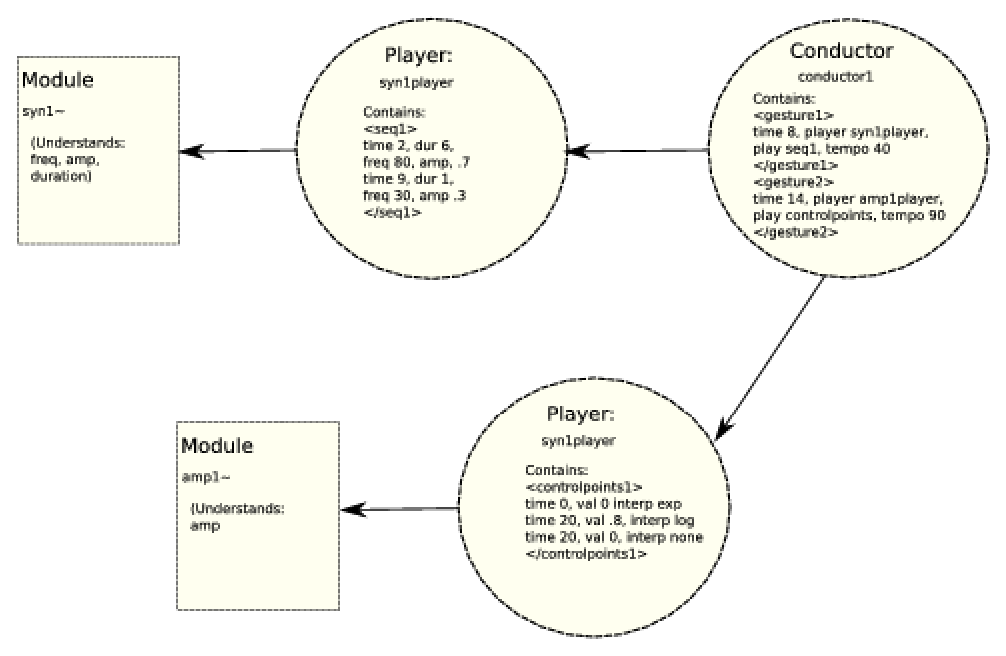
\includegraphics[width=0.9\textwidth]{player-model} %
\caption{A conceptual overview of the conductor-player-module model.}
\end{sidewaysfigure}
%\end{landscape}
%\end{center}

\end{document}
